\documentclass[lualatex]{beamer}
\usepackage[english]{babel}
\usepackage{graphicx}
\usepackage{minted}

\setbeameroption{show notes}
%\setbeameroption{hide notes}
\usetheme{Madrid}

\title[HTTP/2]{An Unpractical Introduction to HTTP/2}
  \author{Taoda}
  \institute{YITU tech}
  \date{Sep\ 2018}

\begin{document}

\begin{frame}
\titlepage
\end{frame}

\begin{frame}
  \frametitle{Outline}
  \tableofcontents
\end{frame}

\section{What is a good protocol?}
\subsection{On the wish list to a below-application-layer protocol}

\begin{frame}
  \frametitle{On the wish list to a below-application-layer protocol}

  \begin{block}{~}
    \begin{itemize}
    \item connectivity
    \item secure: TLS/SSL support
    \item eco-system
    \item explicitly upgradable app-layer: upgrading depends on explicit communications.
    \item high speed
      \begin{itemize}
      \item low overhead on sending data structures
      \item other concerns
      \end{itemize}
    \item multiplexing
    \item tunable: flow control, priority
    \item app-aware health checking
    \end{itemize}
  \end{block}
\end{frame}

\subsection{Some widely adopted protocols}

\begin{frame}
  \frametitle{Some widely adopted protocols}

  \begin{block}{HTTP/1.1}
    \begin{itemize}
    \item best connectivity
    \item secure: HTTPS
    \item eco-system: curl
    \item explicitly upgradable app-layer: accept type/content type
    \item multiplexing: one-way one-shot request-reply model
      \begin{itemize}
      \item pipelining: suffers from head-of-line blocking
      \item connection pool: very heavy burden on the server side
      \end{itemize}
    \item low speed
      \begin{itemize}
      \item low overhead: very redundant headers
      \item cookies is serialized into a header field
      \item suffers from low-start nature of TCP
      \end{itemize}
    \end{itemize}
  \end{block}
\end{frame}

\begin{frame}
  \frametitle{Some widely adopted protocols}

  \begin{block}{Thrift over raw TCP}
    \begin{itemize}
    \item out-of-box usable
    \item almost unconnectable over internet
    \item lack of security
    \item eco-system: bindings to backend languages
    \item implicit upgrade: only thrift compatibility
    \item overhead
      \begin{itemize}
      \item relatively slow in serialization/deserialization
      \item relatively large in size
      \end{itemize}
    \item multiplexing: connection pool
    \item tunable: little can be tuned
    \end{itemize}
  \end{block}
\end{frame}

\begin{frame}
  \frametitle{Some widely adopted protocols}

  \begin{block}{WebSocket}
    \begin{itemize}
    \item defined as a part of HTML5
      \begin{itemize}
      \item to provide a mechanism for \textcolor{red}{browser-based} applications that need \textcolor{blue}{two-way} communication with servers that does \textcolor{green}{not} rely on \textcolor{green}{opening multiple HTTP connections}.
      \end{itemize}
    \item over raw TCP with handshaking over HTTP
    \item TLS/SSL + origin-based security model
    \item implicit upgrading
    \item overhead
      \begin{itemize}
      \item very low overhead: 2-byte in extreme cases
      \end{itemize}
    \item duplexing: two-way streaming
    \item tunable: one purpose per connection. little can/should be tuned.
    \item ping-pong frames with app data
    \end{itemize}
  \end{block}
\end{frame}

\begin{frame}
  \frametitle{Some widely adopted protocols}

  \begin{block}{gRPC}
    \begin{itemize}
    \item gRPC is a RPC library over HTTP/2.
    \item gRPC does not expose HTTP/2 connections.
    \item protobuf is the only choice of serialization.
    \end{itemize}
  \end{block}
\end{frame}

\section{Deep into HTTP/2}

\begin{frame}
  \frametitle{HTTP/2 vs.\ HTTP/1.1}

  \begin{block}{~}
    \begin{center}
      \begin{tabular}{|l|l|l|}
        \hline
        ~& HTTP/1.1 & HTTP/2(rfc7540)\\
        \hline
        connection & one-shot & keep-alive\\
        multiplexing & one-way request-reply & two-way streaming\\
        headers & redundant & HPACK(rfc7541)\\
        cookies & total & incremental\\
        flow control & - & Y\\
        priority & - & Y\\
        \hline
      \end{tabular}
    \end{center}
  \end{block}
\end{frame}

\begin{frame}
  \frametitle{HTTP/2 Architecture}

  \begin{block}{Concepts}
    \begin{itemize}
    \item Connection: a TCP connection with settings.
    \item Frame: the smallest pieces over HTTP/2 connections.
    \item Stream: two-way multiplex data flows
    \end{itemize}
  \end{block}
\end{frame}

\begin{frame}
  \frametitle{Frame}
  \begin{block}{Common format}
    \begin{center}
      \includegraphics{fig/frame_common.pdf}
    \end{center}
  \end{block}
\end{frame}

\subsection{Request-Reply Stream}

\begin{frame}
  \frametitle{Stream}

  \begin{block}{~}
    \begin{itemize}
    \item Multiple concurrently active streams over a same HTTP/2 connection.
    \item Either of peers can establish streams.
    \item The order of frames on a same stream is significant;\\
      that among different streams is controlled by flow-control and priority.
    \item Streams are identified by an integer.
    \item Streams, like TCP, can be half-closed.
    \end{itemize}
  \end{block}
\end{frame}

\begin{frame}
  \frametitle{Stream}

  \begin{block}{Identifiers}
    \begin{itemize}
    \item 31-bit unsigned integers.
    \item odd numbers for client; even numbers for server; 0 for connection.
    \item ID of a newly established stream MUST be greater than IDs of all opened or reserved streams of that endpoint.
    \end{itemize}
  \end{block}
\end{frame}

\subsubsection{Structure}

\begin{frame}
  \frametitle{Request-Reply Stream}

  \begin{block}{Request-Reply Stream}
    \begin{itemize}
    \item Any peer can start a stream, with
      \begin{itemize}
      \item a HEADERS frame
      \item optional CONTINUATION frames to complete headers
      \item optional DATA frames w.r.t.\ HTTP/1.1 body.
      \end{itemize}
    \item The remote peer replies, with the same structure of frames. 
    \end{itemize}
  \end{block}
\end{frame}

\begin{frame}
  \frametitle{Request-Reply Stream}

  \begin{block}{HEADERS(0x1) frame}
    \begin{center}
      \includegraphics{fig/headers_frame.pdf}
    \end{center}
    \begin{itemize}
    \item END\_STREAM(0x1): This is the last frame that this peer will be sent.
    \item END\_HEADERS(0x4): This frame contains entire headers.
    \item PADDED(0x8): Enables the Pad Length and Padding block.
    \item PRIORITY(0x20): Enables the Dependent Stream and Weight block.
    \end{itemize}
  \end{block}
\end{frame}

\begin{frame}
  \frametitle{Request-Reply Stream}

  \begin{block}{CONTINUATION(0x9) frame}
    \begin{center}
      \includegraphics{fig/continuation_frame.pdf}
    \end{center}
    \begin{itemize}
    \item END\_HEADERS(0x4): This is the end of headers.
    \end{itemize}
  \end{block}
\end{frame}

\begin{frame}
  \frametitle{Request-Reply Stream}

  \begin{block}{DATA(0x0) frame}
    \begin{center}
      \includegraphics{fig/data_frame.pdf}
    \end{center}
    \begin{itemize}
    \item END\_STREAM(0x1): Ends a stream.
    \item PADDED(0x8): Enables padding.
    \end{itemize}
  \end{block}
\end{frame}

\subsubsection{Examples}

\begin{frame}[fragile]
  \frametitle{GET request with a small header}

  \begin{columns}[t]
    \begin{column}{.45\textwidth}
      \begin{block}{HTTP/1.1}
        \begin{minted}[gobble=10]{text}
          GET /resource HTTP/1.1
          Host: example.org
          Accept: image/jpg
        \end{minted}
      \end{block}
    \end{column}
    \begin{column}{.45\textwidth}
      \begin{block}{HTTP/2}
        \begin{enumerate}
        \item HEADERS\\+END\_STREAM\\+END\_HEADERS
          \begin{minted}[gobble=12]{text}
            :method = GET
            :scheme = http
            :path = /resource
            host = example.org
            accept = image/jpeg
          \end{minted}
        \end{enumerate}
        The above shows only semantics of headers.
        Syntax is quite different.
      \end{block}
    \end{column}
  \end{columns}
\end{frame}

\begin{frame}[fragile]
  \frametitle{GET response}

  \begin{columns}[t]
    \begin{column}{.45\textwidth}
      \begin{block}{HTTP/1.1}
        \begin{minted}[gobble=10]{text}
          HTTP/1.1 200 OK
          Content-Type: image/jpeg
          Content-Length: 123
          
          (binary data)
        \end{minted}
      \end{block}
    \end{column}
    \begin{column}{0.45\textwidth}
      \begin{block}{HTTP/2}
        \begin{enumerate}
        \item HEADERS\\+END\_HEADERS
          \begin{minted}[gobble=12]{text}
            :status = 200
            content-type = image/jpeg
            content-length = 123
          \end{minted}
        \item DATA\\+END\_STREAM
          \begin{minted}[gobble=12]{text}
            (binary data)
          \end{minted}
        \end{enumerate}
      \end{block}
    \end{column}
  \end{columns}
\end{frame}

\begin{frame}[fragile]
  \frametitle{POST request with a large header}

  \begin{columns}[t]
    \begin{column}{.45\textwidth}
      \begin{block}{HTTP/1.1}
        \begin{minted}[gobble=10]{text}
          POST /resource HTTP/1.1
          Host: example.org
          Content-Type: image/jpeg
          Content-Length: 123
          
          (binary data)
        \end{minted}
      \end{block}
    \end{column}
    \begin{column}{.45\textwidth}
      \begin{block}{HTTP/2}
        \begin{enumerate}
        \item HEADERS
          \begin{minted}[gobble=12]{text}
            :method = POST
            :path = /resource
            :scheme = http
          \end{minted}
        \item CONTINUATION\\+END\_HEADERS
          \begin{minted}[gobble=12]{text}
            content-type = image/jpeg
            host = example.org
            content-length = 123
          \end{minted}
        \item DATA\\+END\_STREAM
          \begin{minted}[gobble=12]{text}
            (binary data)
          \end{minted}
        \end{enumerate}
      \end{block}
    \end{column}
  \end{columns}
\end{frame}

\subsection{Server Push}

\begin{frame}
  \frametitle{Server Push}

  \begin{block}{Server Push}
    \begin{itemize}
    \item Server-push allows, in spite of ``server'' in its name, any peer to pre-emptively send response along with ``promised'' request to another peer.
    \item This is useful when one peer knows the opposite will be interested in something.
    \item A server-push starts with
      \begin{enumerate}
      \item a PUSH\_PROMISE frame
      \item optional CONTINUATION frames
      \item optional DATA frames
      \end{enumerate}
    \end{itemize}
  \end{block}
\end{frame}

\begin{frame}
  \frametitle{Server Push}

  \begin{block}{PUSH-PROMISE(0x5) frame}
    \begin{center}
      \includegraphics{fig/push_promise_frame.pdf}
    \end{center}
  \end{block}
\end{frame}

\subsection{Header Compression}

\begin{frame}
  \frametitle{Header Compression}
  \begin{block}{HPACK}
    \begin{itemize}
    \item HPACK: RFC-7541
    \end{itemize}
  \end{block}
\end{frame}

\subsection{Flow Control}

\begin{frame}
  \frametitle{Flow Control}
  \begin{block}{~}
    \begin{itemize}
    \item borrow-return model
      \begin{itemize}
      \item initializes capacity by SETTINGS frame
      \item consumes capacity by payload of DATA frames
      \item recovers capacity by WINDOW\_UPDATE frames
      \end{itemize}
    \item both stream level and connection level
    \end{itemize}
  \end{block}
\end{frame}

\begin{frame}
  \frametitle{Flow Control}
  \begin{block}{WINDOW\_UPDATE(0x8) frame}
    \begin{center}
      \includegraphics{fig/window_update_frame.pdf}
    \end{center}
    \begin{itemize}
    \item window-size increment is always positive.
    \item stream id indicates the affacted stream; 0 for the entire connection.
    \end{itemize}
  \end{block}
\end{frame}

\subsection{Priority}

\begin{frame}
  \frametitle{Priority}
  \begin{block}{Priority tree}
    \begin{center}
      \includegraphics{fig/priority_tree.pdf}
    \end{center}
    \begin{itemize}
    \item Streams from each peer form a dependency tree with weight.
    \item If A depends on B, A will not be transferred until B is done.
    \item If A and B have a common parent, resources are allocated proportionally on their weight.
    \end{itemize}
  \end{block}
\end{frame}

\begin{frame}
  \frametitle{Priority}
  \begin{block}{PRIORITY(0x2) frame}
    \begin{center}
      \includegraphics{fig/priority_frame.pdf}
    \end{center}
    \begin{itemize}
    \item A stream can attach to the priority tree by HEADERS frame, or restructure by PRIORITY frame.
    \end{itemize}
  \end{block}
\end{frame}

\subsection{Error Handling}

\begin{frame}
  \frametitle{Error Handling}
  \begin{block}{RST\_STREAM(0x3) frame}
    \begin{center}
      \includegraphics{fig/rst_stream_frame.pdf}
    \end{center}
    \begin{itemize}
    \item RST\_STREAM frame fully terminates a stream.
    \end{itemize}
  \end{block}
\end{frame}

\begin{frame}
  \frametitle{Error Handling}
  \begin{block}{GOAWAY(0x7) frame}
    \begin{center}
      \includegraphics{fig/goaway_frame.pdf}
    \end{center}
    \begin{itemize}
    \item Gracefully shutdown a connection and signal serious error conditions.
    \end{itemize}
  \end{block}
\end{frame}

\subsection{Round-trip time}

\begin{frame}
  \frametitle{Round-trip time}
  \begin{block}{PING(0x6) frame}
    \begin{center}
      \includegraphics{fig/ping_frame.pdf}
    \end{center}
    \begin{itemize}
    \item PING frame is designed to measure a minimal RTT.
    \item Once a peer receives a PING, it must immediately response a PING with the same opaque data and ACK flag.
    \end{itemize}
  \end{block}
\end{frame}

\subsection{Settings}

\begin{frame}
  \frametitle{SETTINGS frame}
\end{frame}

\subsection{Connection establishment}

\begin{frame}[fragile]
  \frametitle{Connection establishment}
  \begin{block}{Cleartext with prior knowledge}
    \begin{enumerate}
    \item Client sends a connection preface, followed by a SETTINGS frame\\
      \mint{text}|PRI * HTTP/2.0\r\n\r\nSM\r\n\r\n|
    \item Server responds a connection preface, followed by a SETTINGS frame.
    \item Then a HTTP/2 connection is established.
    \end{enumerate}
  \end{block}
\end{frame}

\begin{frame}
  \frametitle{Connection establishment}
  \begin{block}{Upgrading from HTTP/1.1}
    \begin{center}
      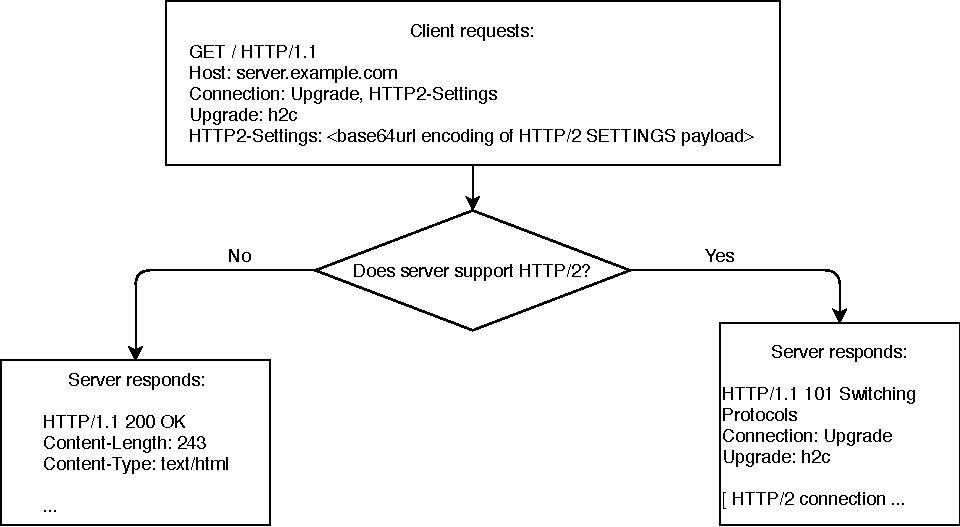
\includegraphics[width=.8\textwidth]{upgrading.pdf}
    \end{center}
    \begin{enumerate}
    \item Server sends a connection preface, followed by a SETTINGS frame.
    \item Client responds a connection preface, followed by a SETTINGS frame.
    \end{enumerate}
  \end{block}
\end{frame}

\begin{frame}
  \frametitle{Connection establishment}
  \begin{block}{HTTPS}
    \begin{enumerate}
    \item Peers negotiate protocol by TLS-ALPN with ``h2''.
    \item Once completing negotiation, both peers must send a connection preface, followed by a SETTINGS frame.
    \end{enumerate}
  \end{block}
\end{frame}

\begin{frame}
  \frametitle{}
  \begin{center}
    \Huge
    Questions?
  \end{center}
\end{frame}

\end{document}
